\documentclass{article}

% NeurIPS 2026, Evaluations and Datasets track.
\usepackage[final,eandd]{neurips_2026}

\usepackage[utf8]{inputenc}
\usepackage[T1]{fontenc}
\usepackage{hyperref}
\usepackage{url}
\usepackage{booktabs}
\usepackage{amsfonts}
\usepackage{amsmath}
\usepackage{amssymb}
\usepackage{microtype}
\usepackage{xcolor}
\usepackage{graphicx}
\usepackage{tikz}
\usetikzlibrary{arrows.meta, positioning, fit, backgrounds}

\graphicspath{{figures/}}

\newcommand{\nlc}{\textsc{nlc}}
\newcommand{\bppi}{\textsc{bppi}}
\newcommand{\nss}{\textsc{nss}}
\newcommand{\ter}{\textsc{ter}}
\newcommand{\nlps}{\textsc{nlps}}
\newcommand{\pqc}{parametrized quantum circuit}
\newcommand{\pqcs}{parametrized quantum circuits}

\title{A Reproducible Evaluation Protocol for Quantum Non-Linearity in Variational Quantum Models}

\author{%
  Pavel Sulimov \\
  Zurich University of Applied Sciences, Zurich \\
  \texttt{suli@zhaw.ch} \\
  \And
  Claude Lehmann \\
  Zurich University of Applied Sciences, Zurich \\
  \texttt{lehl@zhaw.ch} \\
}

\begin{document}
\maketitle

\begin{abstract}
Variational quantum models are linear maps of the input state: any useful non-linearity must be engineered through the data encoding, entanglement pattern, ancilla tracing, classical readouts, or explicit classical layers.
Although many such mechanisms have been proposed, there is no standard protocol that scores them on a common footing.
Most published comparisons reduce non-linearity to either the accuracy on a single downstream benchmark or a single abstract expressibility number, and the two are rarely measured under matched training budgets, circuit widths, and noise assumptions.
We introduce a reproducible evaluation protocol that decomposes non-linearity quality into four complementary scalar scores covering frequency reach, gradient-variance scaling, trainability efficiency on a chaotic dynamical task, and stability under depolarizing noise. In addition, we define a composite index with published weights that sorts methods into rank bands at a fixed operating point $(n,L)$, while preserving full access to the underlying components.
We instantiate the protocol with six variational ans\"atze spanning the standard taxonomy of quantum non-linearity sources (data reuploading, ancilla tracing, their combination, strongly entangling layers, a quantum convolutional network, and a quantum reservoir), together with a classical multilayer perceptron and a hybrid quantum-classical network as non-quantum reference points.
Composite comparisons are within an operating point: repeating the protocol at $(4,4)$ preserves the bottom tier but reorders the top band, so width and depth must be declared and matched.
With fixed tasks, budgets, and seeds, new methods can be added by registering a circuit builder and rerunning the same protocol, and multi-seed aggregates can be updated without changing metric definitions.
\end{abstract}

\section{Introduction}
\label{sec:introduction}

Quantum machine learning studies \pqcs\ (PQCs) as differentiable hypothesis classes that are optimized with classical gradient-based methods and queried through expectation values of chosen observables~\citep{benedetti2019pqcml,cerezo2021cost,bharti2022nisq}.
A central conceptual question in this line of work is whether, and in what sense, \pqcs\ can express non-linear input-output maps.
The joint evolution of a closed quantum system is linear in the state, so any non-linear dependence on classical inputs must be introduced through a specific mechanism: non-linear data encodings~\citep{schuld2021effect,perez2020data}, measurement-induced collapse when classical readouts are taken from entangled registers~\citep{havlicek2019supervised,schuld2019quantum}, ancilla tracing that yields completely-positive trace-preserving channels~\citep{nielsen2010quantum}, or explicit classical post-processing as in hybrid models~\citep{mari2020transfer}.

Despite a growing catalogue of non-linearity mechanisms, empirical evaluation of any newly proposed variational architecture typically takes one of two restricted forms.
Either the architecture is compared through \emph{end-to-end accuracy} on a single downstream benchmark such as Iris or a subset of MNIST~\citep{schuld2020circuit} (which conflates encoding, circuit, readout, optimizer, and dataset size into a single number and rarely controls for the training budget across baselines).
Or it is compared through a \emph{single abstract expressibility or entangling-capability scalar}~\citep{sim2019expressibility} that, by construction, ignores both optimization and readout choices, and does not account for noise or trainability~\citep{mcclean2018barren,holmes2022connecting,ragone2024unified}.
Neither route answers the question that matters when a practitioner proposes a new mechanism for introducing non-linearity into a quantum circuit: at matched circuit width, depth, and training recipe, does the mechanism deliver more Fourier reach, less severe gradient decay, better noise robustness, and better learning efficiency than an established baseline?

We introduce an evaluation protocol that answers this question under the stated constraints.
Our contributions are as follows.
\begin{enumerate}
    \item \textbf{A fixed protocol definition.}
    Four bounded scalar scores — \nlc\ (Fourier reach), \bppi\ (gradient-variance scaling), \nss\ (noise robustness), and \ter\ (trainability efficiency) — measure complementary axes of non-linearity quality under matched width, depth, and training budget.
    A composite \nlps\ with pre-registered weights sorts methods into rank bands at a fixed operating point $(n,L)$; it is reported alongside the four components, never instead of them.
    \item \textbf{A reference evaluation and reusable release.}
    Applying the protocol to six quantum ans\"atze shows quantitatively that composite ranking, Fourier capacity, gradient scaling, noise stability, and held-out regression all disagree on which ansatz is best. The pipeline is released with documented entry points so a new method is added by registering a circuit builder and rerunning the protocol.
\end{enumerate}

\section{Related work}
\label{sec:related}

Early systematic attempts to characterize \pqcs\ introduced the expressibility and entangling-capability scalars of~\citet{sim2019expressibility}, which sample random parameters and measure how close the induced output distribution is to the Haar measure and how strongly the output state is entangled.
These scalars are informative about the \emph{reachable} set of a circuit under random parameters but are explicitly agnostic to the learning problem and to the optimizer: a circuit that is expressive in this sense need not fit a given target function under a finite training budget.
On the optimization side, \citet{mcclean2018barren} showed that gradient variance decays exponentially in qubit count for deep global-cost circuits; follow-up work extended this to local costs~\citep{cerezo2021cost} and showed that high expressibility can itself imply steep gradient decay~\citep{holmes2022connecting,ragone2024unified}.
Our \bppi\ is a bounded cross-method summary of that decay, not a replacement for the per-architecture scaling plots.
Encoding strategies connect directly to function class: \citet{perez2020data} proposed data reuploading and \citet{schuld2021effect} proved that a broad class of single-feature \pqcs\ realizes truncated Fourier series with a spectrum controlled by the encoding; our Non-Linearity Capacity score operationalizes that picture on a geometric ladder of Fourier targets.
Information-theoretic alternatives such as effective dimension via the quantum Fisher information~\citep{abbas2021power} are principled but expensive to estimate at scale; our protocol stays lightweight so the four component scores remain feasible on a laptop for typical benchmark sizes.
Architecturally, \citet{cong2019qcnn} introduced the quantum convolutional network (\textsc{qcnn}); quantum reservoir computing~\citep{fujii2017harnessing,nakajima2019boosting} uses a fixed random unitary and trains only a classical readout - in our registry the closest template to ``encoding plus readout'' without mid-circuit measurement feedback - and hybrid models~\citep{mari2020transfer} add classical non-linear layers on top of a \pqc; we include these templates because they stress whether the protocol discriminates mechanisms rather than merely sizes.
Benchmark suites~\citep{perrier2022qdataset,bowles2024better} standardize data and losses; our goal of standardizing \emph{scoring} of non-linearity quality is orthogonal, since the four axes we evaluate cannot be extracted from a single end-to-end loss.

\section{A protocol for evaluating quantum non-linearity}
\label{sec:protocol}

\subsection{Problem formulation}
\label{sec:problem-formulation}

Let $U(\theta; x)$ be a \pqc\ on $n$ qubits and depth $L$ with trainable parameters $\theta \in \mathbb{R}^P$ and classical input $x$, and let $O$ be an observable used as the readout.
The model output is the scalar expectation
\begin{equation}
    f_\theta(x) = \langle 0^{\otimes n} | U^\dagger(\theta; x) \, O \, U(\theta; x) | 0^{\otimes n} \rangle.
    \label{eq:model}
\end{equation}
A \emph{source of non-linearity} is any concrete mechanism that makes the map $x \mapsto f_\theta(x)$ non-affine in $x$, including but not limited to: non-linear data encodings, repeated data reuploading, ancilla tracing (which yields a channel that is not unitary on the system register), hierarchical structures such as \textsc{qcnn}, fixed random unitaries composed with a trainable readout as in quantum reservoirs, and explicit classical non-linearities in hybrid models.

Given a list of candidate mechanisms, each realized as a choice of $U$, the question we want to answer is the following: at matched width, depth, and training recipe, which mechanism produces a model with the best trade-off between expressive frequency content, trainable gradients, noise tolerance, and learning efficiency?

The protocol fixes the task families, qubit sweeps, noise model, optimizer and budget, global seed, and export format in one place.

The reference registry covers differentiable \pqcs\ with expectation-value readouts.
Four mechanism families fall outside it, for different reasons.
Mid-circuit measurement with feed-forward and post-selection require branching simulation and an accounting convention for discarded shots before a comparison is fair; adding them means a new registry builder rather than a change to the metrics.
A non-linear classical readout is a distinct mechanism; it appears only in the non-competing classical and hybrid reference rows, because scoring it requires a parameter-count convention for classical parameters that we do not fix here.
Quantum kernels without a trainable \pqc\ transfer only partly: \nss\ carries over by freezing the fit and applying the same noise ladder, \nlc\ only under a stated budget convention for closed-form fits, and \bppi\ and \ter\ not at all, since there are no variational parameters or optimization trajectory; such a row would be reported as a separate panel without a composite.
Native open-system training is out of scope; \nss\ applies depolarizing noise after training as a proxy (Section~\ref{sec:limitations}).
In each case the extension path is the same: register a builder and rerun the stages in the fixed order, with metric definitions unchanged (Appendix~\ref{app:ansatz-taxonomy}).
Each scalar is bounded, individually interpretable against prior theory, and accompanied by raw diagnostics in the release; Figure~\ref{fig:metric-intuition} illustrates the geometric construction behind each one.


\begin{table}[t]
  \caption{The four protocol metrics and the composite \nlps\ at a glance. Each row lists the property of a quantum model that the scalar exposes and the raw diagnostic stored alongside it; ``higher is better'' holds for every row, which is why the composite uses $1-\bppi$ rather than \bppi.}
  \label{tab:metric-cheatsheet}
  \centering
  \footnotesize
  \setlength{\tabcolsep}{4pt}
  \begin{tabular}{lp{0.24\linewidth}p{0.22\linewidth}p{0.14\linewidth}p{0.22\linewidth}}
    \toprule
    Metric & Question it answers & Property highlighted & Range & Raw diagnostic \\
    \midrule
    \nlc & How much Fourier frequency content can the model fit under a fixed training budget? & Encoding-driven expressiveness on a $\sin(kx)$ ladder & $[0, 1]$ & Per-rung $R^2_k$ curve \\
    \midrule
    \bppi & How fast does the gradient variance collapse when we add qubits? & Trainability / barren-plateau risk from a \citet{mcclean2018barren}-style probe (default probe loss $f_\theta(0.5)^2$); a plateau-risk verdict, not a fine trainability ranking & $[0, 1]$, lower = healthier; we report $1-\bppi$ & Fitted slope $\alpha$, fit $R^2$, and per-$n$ gradient variances \\
    \midrule
    \nss & How much of the trained fit survives depolarizing noise? & Robustness of a \emph{trained} model to post-gate noise & $[0, 1]$ & $R^2(p)$ at $p\in\{0, 10^{-3}, 5\cdot 10^{-3}, 10^{-2}, 5\cdot 10^{-2}, 10^{-1}\}$ \\
    \midrule
    \ter & How quickly and cheaply does the model learn a small supervised dynamical task? & Optimization efficiency and parameter economy on Lorenz $x_t\to x_{t+1}$ & $\ge 0$ & Train/test $R^2$ vs.\ optimization-step curves and the final test $R^2$ \\
    \midrule
    \nlps & A single-number ranking convenience with fixed convex weights & \emph{Aggregate} non-linearity quality (only meaningful read with components) & $[0, 1]$ & Component vector and effective weights used in~\eqref{eq:nlps-formula} \\
    \bottomrule
  \end{tabular}
\end{table}

\begin{figure}[t]
  \centering
  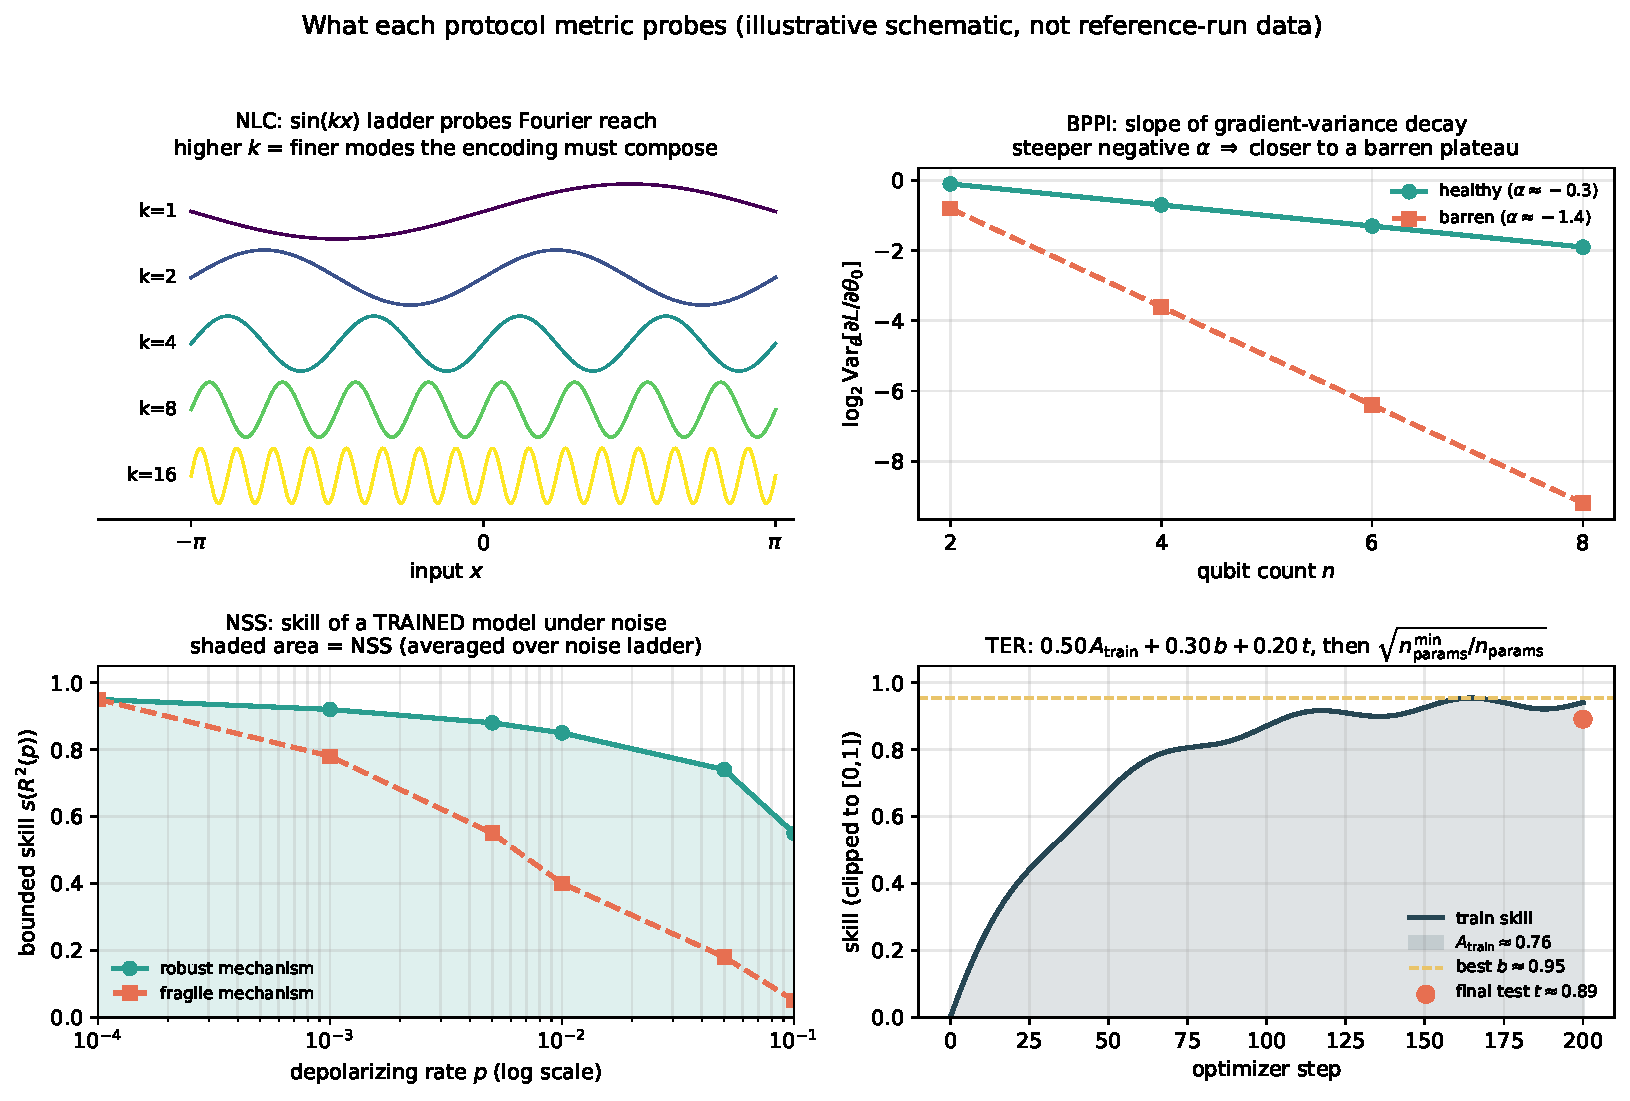
\includegraphics[width=\linewidth]{metric_intuition.pdf}
  \caption{Geometric intuition for the four protocol metrics (illustrative schematic, not reference-run data). \textbf{Top-left:} \nlc\ probes Fourier reach via a $\sin(kx)$ ladder; higher $k$ requires the encoding to compose finer modes. \textbf{Top-right:} \bppi\ measures the slope $\alpha$ of gradient-variance decay across qubit counts; a steeper negative slope signals higher barren-plateau risk. \textbf{Bottom-left:} \nss\ integrates the bounded skill of a \emph{trained} model over a depolarizing noise ladder; the shaded area is the \nss\ value. \textbf{Bottom-right:} \ter\ combines area under the train-skill curve ($A_{\mathrm{train}}$), best train skill ($b$), and final test skill ($t$), scaled by a parameter-economy factor.}
  \label{fig:metric-intuition}
\end{figure}

\subsection{Non-Linearity Capacity}
\label{sec:nlc-definition}

The Non-Linearity Capacity, denoted \nlc, measures how much Fourier frequency content the model can recover under a fixed training budget.
We define a geometric ladder of target functions
\begin{equation}
    f_k(x) = \sin(k\,x), \qquad k \in \{1, 2, 4, 8, 16\}, \qquad x \in [-\pi, \pi],
    \label{eq:nlc-ladder}
\end{equation}
and for each $k$ we train a fresh copy of the model under a fixed optimizer recipe (Adam with learning rate $0.1$, $N_{\mathrm{train}} = 36$ training points, $N_{\mathrm{eval}} = 120$ evaluation points on a grid, a base step budget, and a small per-method boost for a few slow encoders documented in the released metadata file).
We then record the coefficient of determination $R^2_k$ on the evaluation grid and define
\begin{equation}
    \nlc
    \;=\;
    \frac{1}{\log_2 k_{\max}} \int_{0}^{\log_2 k_{\max}}
        \max\!\left(R^2_k(\nu), \, 0\right) \, d\nu,
    \qquad \nu = \log_2 k.
    \label{eq:nlc-formula}
\end{equation}
In practice we compute~\eqref{eq:nlc-formula} by the trapezoidal rule on the ladder in~\eqref{eq:nlc-ladder}.
\nlc\ operationalizes \citet{schuld2021effect}'s Fourier picture on a geometric ladder; the per-$k$ $R^2_k$ curves are exported alongside the scalar.

\subsection{Barren-Plateau Proximity Index}
\label{sec:bppi-definition}

The Barren-Plateau Proximity Index, denoted \bppi, measures how quickly the variance of the loss gradient decays with qubit count and maps it to a bounded plateau-risk scalar.
For each $n \in \{2, 4, 6, 8\}$, we sample $N_{\mathrm{init}}$ random parameter vectors from the same initialization distribution used in the training protocol, fix a probe input $x_{\mathrm{probe}} = 0.5$, and compute
\begin{equation}
    V(n) \;=\; \mathrm{Var}_{\theta}\left[\,\frac{\partial L}{\partial \theta_0}\,\right],
    \label{eq:bppi-variance}
\end{equation}
where $L(\theta) = f_\theta(0.5)^2$ and $\theta_0$ is the first coordinate of $\theta$ in the shared parameter layout (identical index across all methods and all $n$).
We then fit $\log_2 V(n) = \alpha\, n + \beta$ by least squares and define the bounded plateau-risk score
\begin{equation}
    \bppi \;=\; 1 - \exp\!\left(-2 \max(-\alpha,\, 0)\right).
    \label{eq:bppi-formula}
\end{equation}
\bppi\ summarizes \citet{mcclean2018barren}-style gradient-variance decay through the slope $\alpha$; raw $\alpha$, $\beta$, fit $R^2$, and per-$n$ variances are exported.
The cross-method plateau-risk verdict (which method sits at the bottom of $1-\bppi$) is stable under the alternate probe family and the ablation-budget control in Appendix~\ref{app:bppi-probe-ablation}; fine mid-rank orderings are not, so the raw slope remains the preferred audit quantity when comparing to theory.

\subsection{Noise Stability Score}
\label{sec:nss-definition}

The Noise Stability Score, denoted \nss, measures how much of a trained model's regression quality survives depolarizing noise inserted after each gate.
Each model is trained on $y=\sin(x)$ at $p=0$ under the standard $(n,L)$, optimizer, and step budget; training is then frozen.
We then evaluate $R^2(p)$ on a held-out grid under single-qubit depolarizing noise at rates $p \in \{0, 10^{-3}, 5 \cdot 10^{-3}, 10^{-2}, 5 \cdot 10^{-2}, 10^{-1}\}$.
We convert each $R^2$ to a bounded skill score
\begin{equation}
    s(R^2) \;=\; \max\!\left(\min\!\left(\frac{R^2 + 1}{2}, 1\right), 0\right) \in [0, 1],
\end{equation}
and integrate
\begin{equation}
    \nss
    \;=\;
    \frac{1}{p_{\max} - p_{\min}}
    \int_{p_{\min}}^{p_{\max}} s\!\left(R^2(p)\right) \, dp
    \;\approx\;
    \text{trapezoid on the grid above}.
    \label{eq:nss-formula}
\end{equation}
Integrating over the noise ladder captures both early and late degradation; raw $R^2(p)$ curves distinguish a weak clean fit from rapid collapse.

\subsection{Trainability Efficiency Ratio}
\label{sec:ter-definition}

The Trainability Efficiency Ratio, denoted \ter, measures how efficiently the model learns the Lorenz \emph{one-step} prediction task.
Mackey-Glass is used later as a chaotic regression stress test under the same Pauli readout.
Throughout, ``one-step'' refers to the supervised target $(x_t, x_{t+1})$; the optimization-step axis underlies $A_{\mathrm{train}}$, while Figure~\ref{fig:lorenz-pred}'s x-axis is the independent test-window index.
Given the Lorenz~\citep{lorenz1963} trajectory $\{x_t\}$, we form supervised pairs $(x_t, x_{t+1})$ from a transient-free window of length $N_{\mathrm{train}}$, train each model with Adam for $N_{\mathrm{steps}}$ optimization steps and evaluate every $N_{\mathrm{eval}}$ of them, and record the train and test $R^2$ curves over that optimization-step axis.
Let $A_{\mathrm{train}}$ be the area under the clipped train-skill curve (integrated in step index and normalized to $[0, 1]$), let $b$ be the best train-skill value attained, let $t$ be the test skill at the final step, and let $n_{\mathrm{params}}$ be the number of trainable parameters.
We define
\begin{equation}
    \ter
    \;=\;
    \Bigl(\,
        0.50 \cdot A_{\mathrm{train}}
        +
        0.30 \cdot b
        +
        0.20 \cdot t
    \,\Bigr)
    \,\cdot\,
    \sqrt{\frac{n_{\mathrm{params}}^{\min}}{n_{\mathrm{params}}}},
    \label{eq:ter-formula}
\end{equation}
where $n_{\mathrm{params}}^{\min}$ is the smallest parameter count across the current registry of methods.
The $(0.50, 0.30, 0.20)$ split and parameter multiplier are fixed design choices recorded in the released metadata; full train curves are exported.

\subsection{Composite score}
\label{sec:nlps-definition}

We finally aggregate the four protocol scores into a single benchmark-level index, which we call the Non-Linearity Protocol Score and denote \nlps.
It is defined by the fixed convex combination
\begin{equation}
    \nlps
    \;=\;
    0.35 \cdot \nlc
    \;+\;
    0.25 \cdot (1 - \bppi)
    \;+\;
    0.20 \cdot \ter
    \;+\;
    0.20 \cdot \nss.
    \label{eq:nlps-formula}
\end{equation}
The convex weights $(0.35, 0.25, 0.20, 0.20)$ for $(\nlc, 1-\bppi, \ter, \nss)$ are a \emph{fixed multi-criteria convention} that is frozen with the release.
They encode the priority ordering implicit in the protocol definition: \nlc\ receives the largest coefficient because it is the only component that directly probes non-linearity through Fourier reach; $1-\bppi$ receives the next largest coefficient because a mechanism that cannot maintain trainable gradients is unlikely to scale; \ter\ and \nss\ enter symmetrically as practical deployment probes, one for optimization efficiency on a chaotic supervised task and one for hardware-noise robustness.
The numerical vector should be read as a transparent encoding of those priorities, not as an empirically fitted optimum.
Formal preference-elicitation schemes such as the Analytic Hierarchy Process~\citep{saaty1987ahp} could be used to replace these weights in a separate benchmark variant, but doing so would require independent pairwise judgments before looking at the reference results.
We therefore do not tune the weights by grid search on the reference tables, which would leak information from the evaluated methods into the scoring rule.

We invert \bppi\ as $1-\bppi$ so that larger values consistently correspond to better performance across all metrics. \nlps\ remains a ranking convenience, not a utility function. Two methods with the same \nlps\ can differ sharply on components or on any given downstream task (Section~\ref{sec:metric-divergence}).
Close \nlps\ scores should be read as rank bands.
The weight-sensitivity analysis (Appendix~\ref{app:weight-sensitivity}) supports this reading: over $10^5$ admissible weight vectors drawn within the stated priority ordering, the top two ranks never change and the mean Kendall $\tau$ against the published ranking is $0.974$ ($0.982$ under local perturbations with $\|w-w^{(0)}\|_\infty \le 0.10$); the nearest possible rank tie, between ancilla reuploading and \textsc{qcnn}, requires $\|w-w^{(0)}\|_\infty \approx 0.015$.
Robustness to the weighting does not extend to the operating point: rank bands are defined only within a declared $(n,L)$ (Section~\ref{sec:evaluation-protocol}, Appendix~\ref{app:scaling-n4-l4}).

\paragraph{Intended use of the composite.}
\nlps\ gives methods evaluated at the same width and depth a common, pre-registered axis, so that four-component results from separate papers can be placed side by side without each author choosing a weighting after seeing their own numbers.
It sorts methods into rank bands, not places, and it is meaningful only next to the component table.
It is not a utility function and not a substitute for evaluating a candidate on the practitioner's own task: across the six reference ans\"atze, the rank correlation between \nlps\ and held-out Lorenz $R^2$ is $0.03$ (Section~\ref{sec:metric-divergence}).
Where the components disagree, the components are the result.

\section{Evaluation protocol for new methods}
\label{sec:evaluation-protocol}

To evaluate a new method, register a circuit builder with its parameter shape in the shared method registry; no scoring code needs to be modified.
The pipeline runs four stages in sequence and aggregates them into the composite \nlps\ via~\eqref{eq:nlps-formula}; optional real-data and hybrid stages follow without feeding back into \nlps.
The released configuration is organized as follows.
\begin{itemize}
  \item \textbf{Registry interface.} A circuit builder defining $U(\theta; x)$ and its parameter shape is registered once; all stages read from this registry at runtime and share the same global seed.
  \item \textbf{Stage order.} Stages execute as \nlc\ $\to$ \bppi\ $\to$ \nss\ $\to$ \ter\ $\to$ composite, with per-stage hyperparameters fixed in Appendix~\ref{app:reproducibility}.
  \item \textbf{Fixed vs.\ free.} The Fourier ladder, qubit sweep, noise ladder, optimizer, evaluation cadence, composite weights, and global seed are fixed.
  Circuit width $n$ and depth $L$ are free design choices but must be declared and matched across compared methods: \nlps\ values from different $(n,L)$ are not comparable (Appendix~\ref{app:scaling-n4-l4}).
  The readout observable and non-linearity mechanism remain free.
\end{itemize}

\section{Reference evaluation}
\label{sec:results}

We apply the protocol to six variational ans\"atze that cover the standard taxonomy of non-linearity mechanisms. This verifies that the protocol runs end-to-end and demonstrates that the metrics can disagree on which ansatz is best, motivating separate reporting.

\subsection{Methods and setup}
\label{sec:methods}

Table~\ref{tab:registry} lists the six quantum ans\"atze together with a classical multilayer perceptron and a hybrid quantum-classical reference.
The quantum ans\"atze were chosen so that each isolates a different source of non-linearity: encoding only (data reuploading), channel only (ancilla tracing), both together (ancilla reuploading), hardware-efficient entanglement (strongly entangling layers), hierarchical structure (\textsc{qcnn}), and fixed random dynamics with trainable classical readout (quantum reservoir).
The six rows are therefore a spanning set over mechanism types rather than a survey of published architectures; a further row is warranted when it introduces a mechanism not already represented, which is the case the registry interface is built for.

\begin{table}[t]
  \caption{Methods included in the reference evaluation and the source of non-linearity each isolates. Dashes in the parameter column mark classical baselines whose widths are set by the hybrid and real-data stages and are not matched to the six quantum counts.}
  \label{tab:registry}
  \centering
  \small
  \resizebox{\textwidth}{!}{
  \begin{tabular}{llr}
    \toprule
    Method & Non-linearity mechanism & Trainable parameters \\
    \midrule
    Strongly entangling layers                        & Entanglement baseline                      & 27 \\
    Data reuploading~\citep{perez2020data}            & Re-injected encoding                       & 18 \\
    Ancilla tracing                                   & Partial trace (channel)                    & 18 \\
    Ancilla reuploading                               & Encoding + channel (combined)              & 18 \\
    Quantum convolutional network~\citep{cong2019qcnn}& Hierarchical structure                     & 12 \\
    Quantum reservoir~\citep{fujii2017harnessing}     & Fixed unitary + classical readout          & 6 \\
    \midrule
    Classical MLP (2 hidden layers)                   & Classical activations                      & - \\
    Hybrid quantum-classical network~\citep{mari2020transfer} & Circuit + classical layer         & - \\
    \bottomrule
  \end{tabular}
  }
\end{table}

All stages share the same simulator backend and global seed; per-stage hyperparameters are listed in Appendix~\ref{app:reproducibility}.

Full protocol at $(n,L)=(3,3)$ runs in approximately two hours wall-time on an 8-core CPU; details in Appendix~\ref{app:reproducibility}.
Simulation uses PennyLane~\citep{bergholm2018pennylane} (Apache~2.0) and scikit-learn~\citep{pedregosa2011scikitlearn} (BSD-3-Clause); full asset list in Appendix~\ref{app:reproducibility}.

\subsection{Protocol metrics and composite ranking}
\label{sec:protocol-results}

Table~\ref{tab:nlps-components} reports the four protocol metrics and the composite index for each quantum ansatz at the reference operating point $(n,L)=(3,3)$.
Data reuploading attains the highest \nlps\ under the published weights, consistent with its well-known Fourier reach; ancilla tracing and ancilla reuploading attain near-perfect plateau-risk scores ($1 - \bppi$ of $0.99$ and $0.94$), while strongly entangling layers collapse on both $1 - \bppi$ and \nss.
Monte Carlo over $10^5$ admissible weight vectors keeps the top-2 \nlps\ ranks fixed and yields Kendall $\tau = 0.974$ with the published ranking; ancilla reuploading and \textsc{qcnn} occupy a 3--4 rank band.
Local-$\varepsilon$ analysis and \ter-only resampling are in Appendix~\ref{app:weight-sensitivity}.
Rank bands are therefore robust to the weighting at fixed $(n,L)$, but not to the operating point: repeating the full protocol at $(4,4)$ with the same budgets and $K=5$ seeds gives Kendall $\tau = 0.60$ against $(3,3)$, with the bottom two ranks unchanged and the composite leader flipping to ancilla reuploading (Appendix~\ref{app:scaling-n4-l4}).
Probe-loss sensitivity of $1-\bppi$ is reported in Appendix~\ref{app:bppi-probe-ablation}.

\begin{table}[t]
  \caption{Protocol components and composite \nlps\ per quantum ansatz (higher is better in all columns). \protectMean $\pm$ one standard deviation over $K=5$ protocol runs (\texttt{QNLEP\_SEED} $\in \{42, 43, 44, 45, 46\}$). Bold marks the highest mean per column \emph{among quantum rows only}; classical reference rows are shown below the midrule and are never bolded.
}
  \label{tab:nlps-components}
  \centering
  \small
  \setlength{\tabcolsep}{6pt}
  \resizebox{\textwidth}{!}{
  \begin{tabular}{lrrrrr}
    \toprule
    Method & \nlc & $1 - \bppi$ & \ter & \nss & \nlps \\
    \midrule
        Strongly entangling (baseline) & 0.368 $\pm$ 0.001 & 0.029 $\pm$ 0.005 & 0.123 $\pm$ 0.003 & 0.338 $\pm$ 0.122 & 0.228 $\pm$ 0.024 \\
    Data reuploading       & \textbf{0.437 $\pm$ 0.023} & 0.876 $\pm$ 0.064 & 0.073 $\pm$ 0.022 & \textbf{0.902 $\pm$ 0.007} & \textbf{0.567 $\pm$ 0.021} \\
    Ancilla tracing        & 0.307 $\pm$ 0.003 & \textbf{0.988 $\pm$ 0.021} & 0.088 $\pm$ 0.006 & 0.893 $\pm$ 0.011 & 0.551 $\pm$ 0.005 \\
    Ancilla reuploading    & 0.261 $\pm$ 0.005 & 0.938 $\pm$ 0.037 & \textbf{0.151 $\pm$ 0.001} & 0.673 $\pm$ 0.005 & 0.491 $\pm$ 0.010 \\
    Quantum CNN            & 0.292 $\pm$ 0.018 & 0.662 $\pm$ 0.083 & 0.121 $\pm$ 0.006 & 0.890 $\pm$ 0.034 & 0.470 $\pm$ 0.018 \\
    Quantum reservoir      & 0.087 $\pm$ 0.041 & 0.311 $\pm$ 0.409 & 0.009 $\pm$ 0.016 & 0.517 $\pm$ 0.108 & 0.213 $\pm$ 0.109 \\

    % Ensure a row break before booktabs rule even if generated body omits final \\.
    \\
    \bottomrule
  \end{tabular}
  }
\end{table}

\subsection{Lorenz one-step prediction}
\label{sec:lorenz-results}

Table~\ref{tab:lorenz-r2} reports held-out $R^2$ for Lorenz one-step regression, on the same trained models used to compute \ter.
The best forecaster is ancilla reuploading, followed by \textsc{qcnn} and strongly entangling layers; data reuploading, the composite \nlps\ leader, is near-zero on this task.

\begin{table}[t]
  \caption{Held-out $R^2$ on the Lorenz one-step prediction task, evaluated on the same trained models used to compute \ter. Higher is better; negative values indicate worse-than-mean predictions. \protectMean $\pm$ one standard deviation over $K=5$ protocol runs (\texttt{QNLEP\_SEED} $\in \{42, 43, 44, 45, 46\}$). Bold marks the highest mean per column \emph{among quantum rows only}; classical reference rows are shown below the midrule and are never bolded.
}
  \label{tab:lorenz-r2}
  \centering
  \small
  \begin{tabular}{lr}
    \toprule
    Method & Test $R^2$ \\
    \midrule
    Strongly entangling (baseline) & 0.436 $\pm$ 0.031 \\
    Data reuploading       & -0.118 $\pm$ 0.132 \\
    Ancilla tracing        & 0.375 $\pm$ 0.020 \\
    Ancilla reuploading    & \textbf{0.477 $\pm$ 0.000} \\
    Quantum CNN            & 0.403 $\pm$ 0.025 \\
    Quantum reservoir      & -1.099 $\pm$ 0.357 \\

    \\
    \bottomrule
  \end{tabular}
\end{table}

\begin{figure}[t]
  \centering
  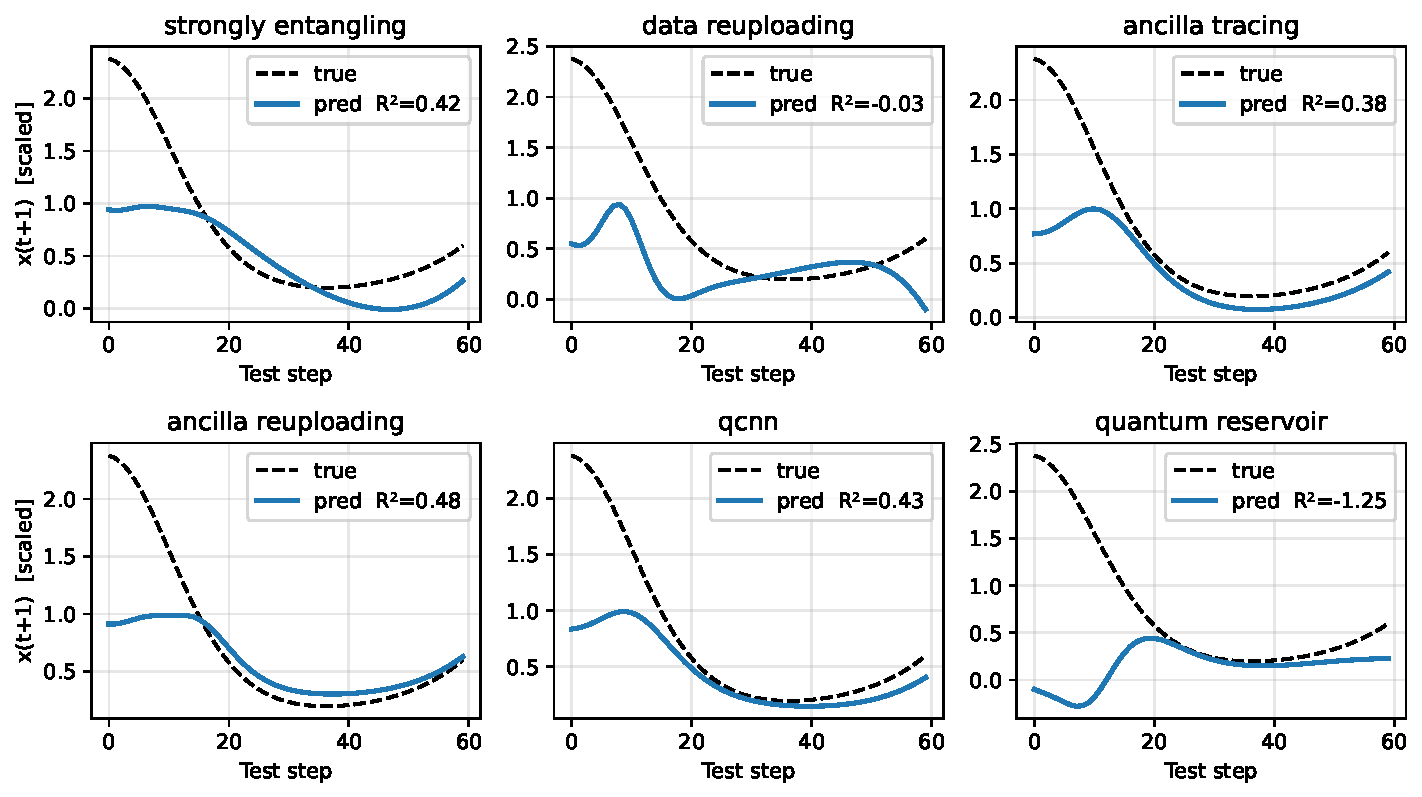
\includegraphics[width=\linewidth]{lorenz_predictions.pdf}
  \caption{Representative Lorenz \emph{one-step} predictions. Each point on the horizontal axis is an independent supervised prediction $\hat x_{t+1} = f_\theta(x_t)$ for a different test index $t$; the x-axis is therefore the test-window \emph{time index}, not a multi-step roll-out or the training-step axis of \ter. Although data reuploading is the composite \nlps\ leader (Table~\ref{tab:nlps-components}), its one-step prediction collapses on the test window, while ancilla reuploading, \textsc{qcnn}, and strongly entangling layers produce visibly correct trajectories.}
  \label{fig:lorenz-pred}
\end{figure}

\subsection{Elementary classification and regression benchmarks}
\label{sec:real-data-results}

Table~\ref{tab:real-data} reports results from the released real-data evaluation stage, which applies the same trained-from-scratch recipe to three binary classification tasks (\textsc{circles}, \textsc{moons}, and an Iris subset restricted to classes $1$ and $2$) and two regression tasks ($f(x) = x\sin(x)$ with regression targets scaled to $[-1, 1]$ to match a single Pauli-$Z$ readout range, and one-step Mackey-Glass forecasting with the same readout).
How these columns relate to the protocol scores is analysed in Section~\ref{sec:metric-divergence}.

\begin{table}[t]
  \caption{Real-data scores from the released evaluation. Classification columns report test accuracy in $[0,1]$; regression columns report test $R^2$ (higher is better; values below zero mean worse than predicting the training mean). Mackey-Glass one-step forecasting is a deliberately hard chaotic regression under a single Pauli-$Z$ readout: every model attains large negative $R^2$, so the column is a stress test where ``best'' means least negative. The $x\sin(x)$ task is a smoother one-dimensional map with targets scaled to the readout range. Quantum rows (including ancilla reuploading) are reported above the midrule; the row labelled \emph{Strongly entangling (baseline)} is a hardware-efficient PQC (Strongly-Entangling-Layers with a single angle encoding, no re-uploading and no ancilla tricks) and plays the role of a \emph{simple quantum baseline}. Below the midrule, the classical MLP and the hybrid QCNN use classical capacity that pure PQCs do not; those rows are non-competing references and are never bolded; bold marks the best value among the quantum rows only. \protectMean $\pm$ one standard deviation over $K=5$ protocol runs (\texttt{QNLEP\_SEED} $\in \{42, 43, 44, 45, 46\}$). Bold marks the highest mean per column \emph{among quantum rows only}; classical reference rows are shown below the midrule and are never bolded.
}
  \label{tab:real-data}
  \centering
  \small
  \setlength{\tabcolsep}{5pt}
  \begin{tabular}{lccccc}
    \toprule
      & \multicolumn{3}{c}{Classification (accuracy $\uparrow$)} & \multicolumn{2}{c}{Regression ($R^2$ $\uparrow$)} \\
    \cmidrule(lr){2-4}\cmidrule(lr){5-6}
    Method & Circles & Moons & Iris (1v2) & $x\sin(x)$ & Mackey-Glass \\
    \midrule
    Strongly entangling (baseline) & 0.69 $\pm$ 0.10 & 0.73 $\pm$ 0.00 & 0.67 $\pm$ 0.00 & \textbf{0.89 $\pm$ 0.01} & -362 $\pm$ 4 \\
    Data reuploading         & 0.72 $\pm$ 0.02 & \textbf{0.77 $\pm$ 0.01} & 0.63 $\pm$ 0.01 & 0.72 $\pm$ 0.03 & \textbf{-346 $\pm$ 10} \\
    Ancilla tracing          & 0.74 $\pm$ 0.02 & 0.73 $\pm$ 0.03 & \textbf{0.69 $\pm$ 0.03} & 0.65 $\pm$ 0.02 & -381 $\pm$ 4 \\
    Ancilla reuploading      & 0.68 $\pm$ 0.03 & 0.73 $\pm$ 0.03 & 0.60 $\pm$ 0.10 & 0.45 $\pm$ 0.04 & -389 $\pm$ 55 \\
    Quantum CNN              & \textbf{0.75 $\pm$ 0.00} & 0.71 $\pm$ 0.04 & 0.64 $\pm$ 0.01 & 0.83 $\pm$ 0.01 & -372 $\pm$ 7 \\
    Quantum reservoir        & \textbf{0.75 $\pm$ 0.00} & 0.40 $\pm$ 0.00 & 0.67 $\pm$ 0.00 & 0.46 $\pm$ 0.00 & -398 $\pm$ 6 \\
    \midrule
    Classical MLP (ref.)     & 1.00 $\pm$ 0.01 & 1.00 $\pm$ 0.00 & 0.91 $\pm$ 0.01 & 0.95 $\pm$ 0.06 & -339 $\pm$ 152 \\
    Hybrid QCNN (ref.)       & 0.72 $\pm$ 0.03 & 0.71 $\pm$ 0.05 & 0.59 $\pm$ 0.02 & 0.99 $\pm$ 0.00 & -3 $\pm$ 4 \\

    \\
    \bottomrule
  \end{tabular}
\end{table}

\begin{figure}[t]
  \centering
  \begin{minipage}[c]{0.46\linewidth}
    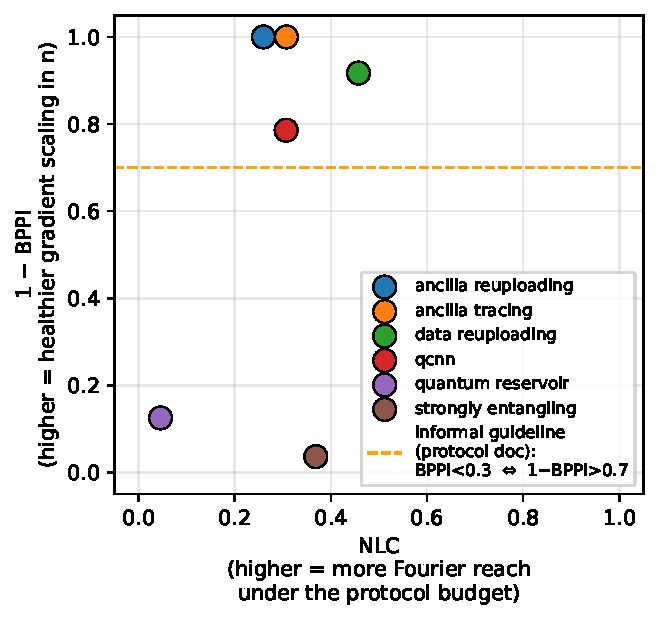
\includegraphics[width=\linewidth]{nlc_vs_bppi_scatter.pdf}
  \end{minipage}\hfill
  \begin{minipage}[c]{0.51\linewidth}
  \caption{\nlc\ versus $1 - \bppi$ for each quantum ansatz (both axes ``higher is better'' within the protocol). No method lies in the upper-right corner with simultaneously maximal Fourier reach and maximal gradient health; ancilla-based points cluster toward safer $1-\bppi$ at moderate \nlc, while strongly entangling layers trade gradient scaling for frequency reach. The dashed line is the optional $\bppi<0.3$ guideline from the protocol text, not a hard partition used in scoring.}
  \label{fig:nlc-vs-bppi}
  \end{minipage}
\end{figure}

\subsection{Empirical metric divergence}
\label{sec:metric-divergence}

The central empirical observation of this paper is that no single metric orders the six ans\"atze consistently with the others.
Data reuploading leads on \nlps\ but ranks next-to-worst on Lorenz $R^2$; ancilla reuploading reverses that ordering.
Strongly entangling layers carry the highest \bppi\ risk consistent with~\citet{holmes2022connecting}, despite a middling \nlc; the quantum reservoir ranks last on \nlps\ and Lorenz $R^2$ but is middling on classification, consistent with a randomized feature-map interpretation.
None of these observations can be read off a single number; all fall out immediately from the component view enforced by the protocol.

\paragraph{Protocol scores versus downstream tasks.}
Rank correlations between the protocol scalars and the downstream columns of Tables~\ref{tab:lorenz-r2} and~\ref{tab:real-data} (Spearman $\rho$ over the six method-level means at $(3,3)$, $K=5$ seeds; full matrix in Table~\ref{tab:downstream-correlation}) show that each component tracks the task family it was designed around and little beyond it.
\nlc, which probes Fourier reach, tracks \textsc{moons} accuracy ($\rho = 0.81$) and $x\sin x$ regression ($\rho = 0.66$); \nlps\ does not track Lorenz $R^2$ ($\rho = 0.03$).
\ter\ orders the Lorenz column exactly ($\rho = 1.00$), but this is a consistency check rather than evidence of predictive power, because \ter\ and the Lorenz column are computed from the same trained models.
With six methods per correlation we read the pattern rather than the effect sizes; the Mackey--Glass column is a stress case in which every model is far below the mean baseline, so correlations with it separate degrees of failure rather than quality.
The protocol scores are therefore task-family probes, not a ranking that can replace evaluation on the practitioner's own task.

Figure~\ref{fig:nlc-vs-bppi} plots \nlc\ against $1 - \bppi$ (the same orientation as the composite score) and illustrates the expressibility-trainability tension of~\citet{holmes2022connecting}: strongly entangling layers sit toward high \nlc\ but low $1-\bppi$, while ancilla-based mechanisms occupy the opposite corner.

\section{Discussion}
\label{sec:discussion}

\paragraph{Role of \nlps.}
\nlps\ is a frozen leaderboard convention for methods compared at the same $(n,L)$, read in rank bands and only next to the component table (Section~\ref{sec:nlps-definition}).
The metric-divergence result in Section~\ref{sec:metric-divergence} is therefore evidence \emph{for} multi-metric reporting, not an argument against publishing a composite at all.

When proposing a new non-linearity mechanism, the protocol gives a concrete recipe for a fair comparison: evaluate it alongside at least one established mechanism from Table~\ref{tab:registry} at matched $(n, L)$, then report the four component scores and \nlps\ together.
A mechanism that increases \nlc\ at the cost of a larger \bppi\ is an important finding (expressibility-trainability trade-off), as is a mechanism that increases \nss\ without harming \nlc\ (noise-friendly expressiveness); reporting only \nlps\ without the components would hide the information the protocol is built to expose.
The results are consistent with prior predictions~\citep{perez2020data,schuld2021effect,mcclean2018barren,holmes2022connecting}: data reuploading achieves the highest \nlc, strongly entangling layers carry the highest \bppi\ risk, and ancilla tracing trains at moderate depth without visible plateau risk.
The hybrid QCNN reference row (near-ceiling $x\sin(x)$ regression, least-negative Mackey-Glass $R^2$) shows that classical post-processing remains a competitive baseline.

\section{Limitations}
\label{sec:limitations}

Mid-circuit measurements with classical feed-forward are plausible non-linearity sources but are excluded from the reference tables for the simulator and accounting reasons stated in Section~\ref{sec:problem-formulation}; extending the protocol to them is future work once builders and noise models stabilize.
All four scores hold the training recipe fixed across methods, so a method that would eventually fit a high-frequency ladder target with a larger budget still registers as a \nlc\ failure under the protocol budget; this is intentional for comparability.
\nss\ uses depolarizing noise inserted after each gate as a standard simulation proxy; real hardware exhibits coherent and correlated errors that such channels do not capture, so hardware-matched noise models are a natural extension.
The reference run uses $(n, L) = (3, 3)$ as the primary operating point; Appendix~\ref{app:scaling-n4-l4} repeats the full protocol at $(4, 4)$ and finds that composite rank bands are not stable under that change (Kendall $\tau = 0.60$), so \nlps\ comparisons must stay within a declared operating point.
\bppi\ probe choice affects fine mid-rank orderings but not the plateau-risk verdict (Appendix~\ref{app:bppi-probe-ablation}).
Larger qubit counts are used only during the \bppi\ sweep at fixed reference depth.


\section{Conclusion}
\label{sec:conclusion}

We fixed a four-metric plus composite protocol for comparing quantum non-linearity mechanisms under matched training and width conventions, with machine-readable diagnostics per score.
The reference run shows that rankings shuffle across metrics and simple downstream panels (Section~\ref{sec:metric-divergence}); stage ordering and reproducibility details are in Appendix~\ref{app:reproducibility}.
As to broader impact, the protocol is an evaluation tool for a pre-deployment research community; we are not aware of dual-use concerns specific to it.

\section*{Acknowledgements and disclosures}

We thank the two anonymous reviewers and the area chair for the discussion that led to the operating-point and probe-ablation controls in Appendices~\ref{app:bppi-probe-ablation} and~\ref{app:scaling-n4-l4}.

\paragraph{Funding and competing interests.}
This work was partially funded by the Institute of Computer Science at Zurich University of Applied Sciences through the project \textnumero\,79838 ``QML -- Quantum Machine Learning''~\citep{zhaw2026qml}. The authors declare no competing interests.

%\section*{References}
\newpage
{
\small
\begin{thebibliography}{99}

\bibitem[Abbas et~al.(2021)]{abbas2021power}
A.~Abbas, D.~Sutter, C.~Zoufal, A.~Lucchi, A.~Figalli, and S.~Woerner.
\newblock The power of quantum neural networks.
\newblock \emph{Nature Computational Science}, 1(6):403-409, 2021.

\bibitem[Bergholm et~al.(2018)]{bergholm2018pennylane}
V.~Bergholm, J.~Izaac, M.~Schuld, C.~Gogolin, S.~Ahmed, V.~Ajith, M.~S.~Alam, G.~Alonso-Linaje, B.~AkashNarayanan, A.~Asadi, et~al.
\newblock PennyLane: Automatic differentiation of hybrid quantum-classical computations.
\newblock \emph{arXiv preprint arXiv:1811.04968}, 2018.

\bibitem[Benedetti et~al.(2019)]{benedetti2019pqcml}
M.~Benedetti, E.~Lloyd, S.~Sack, and M.~Fiorentini.
\newblock Parameterized quantum circuits as machine learning models.
\newblock \emph{Quantum Science and Technology}, 4(4):043001, 2019.

\bibitem[Bharti et~al.(2022)]{bharti2022nisq}
K.~Bharti, A.~Cervera-Lierta, T.~H. Kyaw, T.~Haug, S.~Alperin-Lea, A.~Anand, M.~Degroote, H.~Heimonen, J.~S. Kottmann, T.~Menke, W.-K. Mok, S.~Sim, L.-C.~Kwek, and A.~Aspuru-Guzik.
\newblock Noisy intermediate-scale quantum (NISQ) algorithms.
\newblock \emph{Reviews of Modern Physics}, 94:015004, 2022.

\bibitem[Bowles et~al.(2024)]{bowles2024better}
J.~Bowles, S.~Ahmed, and M.~Schuld.
\newblock Better than classical? The subtle art of benchmarking quantum machine learning models.
\newblock \emph{arXiv preprint arXiv:2403.07059}, 2024.

\bibitem[Cerezo et~al.(2021)]{cerezo2021cost}
M.~Cerezo, A.~Arrasmith, R.~Babbush, S.~C.~Benjamin, S.~Endo, K.~Fujii, J.~R.~McClean, K.~Mitarai, X.~Yuan, L.~Cincio, and P.~J.~Coles.
\newblock Variational quantum algorithms.
\newblock \emph{Nature Reviews Physics}, 3:625-644, 2021.

\bibitem[Cong et~al.(2019)]{cong2019qcnn}
I.~Cong, S.~Choi, and M.~D. Lukin.
\newblock Quantum convolutional neural networks.
\newblock \emph{Nature Physics}, 15:1273-1278, 2019.

\bibitem[Fujii and Nakajima(2017)]{fujii2017harnessing}
K.~Fujii and K.~Nakajima.
\newblock Harnessing disordered-ensemble quantum dynamics for machine learning.
\newblock \emph{Physical Review Applied}, 8:024030, 2017.

\bibitem[Havl\'i\v{c}ek et~al.(2019)]{havlicek2019supervised}
V.~Havl\'i\v{c}ek, A.~D. C\'orcoles, K.~Temme, A.~W. Harrow, A.~Kandala, J.~M. Chow, and J.~M. Gambetta.
\newblock Supervised learning with quantum-enhanced feature spaces.
\newblock \emph{Nature}, 567:209-212, 2019.

\bibitem[Holmes et~al.(2022)]{holmes2022connecting}
Z.~Holmes, K.~Sharma, M.~Cerezo, and P.~J.~Coles.
\newblock Connecting ansatz expressibility to gradient magnitudes and barren plateaus.
\newblock \emph{PRX Quantum}, 3:010313, 2022.

\bibitem[Lorenz(1963)]{lorenz1963}
E.~N. Lorenz.
\newblock Deterministic nonperiodic flow.
\newblock \emph{Journal of the Atmospheric Sciences}, 20(2):130-141, 1963.

\bibitem[Mackey and Glass(1977)]{mackeyglass1977}
M.~C. Mackey and L.~Glass.
\newblock Oscillation and chaos in physiological control systems.
\newblock \emph{Science}, 197(4300):287-289, 1977.

\bibitem[Mari et~al.(2020)]{mari2020transfer}
A.~Mari, T.~R. Bromley, J.~Izaac, M.~Schuld, and N.~Killoran.
\newblock Transfer learning in hybrid classical-quantum neural networks.
\newblock \emph{Quantum}, 4:340, 2020.

\bibitem[McClean et~al.(2018)]{mcclean2018barren}
J.~R.~McClean, S.~Boixo, V.~N.~Smelyanskiy, R.~Babbush, and H.~Neven.
\newblock Barren plateaus in quantum neural network training landscapes.
\newblock \emph{Nature Communications}, 9:4812, 2018.

\bibitem[Nakajima et~al.(2019)]{nakajima2019boosting}
K.~Nakajima, K.~Fujii, M.~Negoro, K.~Mitarai, and M.~Kitagawa.
\newblock Boosting computational power through spatial multiplexing in quantum reservoir computing.
\newblock \emph{Physical Review Applied}, 11:034021, 2019.

\bibitem[Nielsen and Chuang(2010)]{nielsen2010quantum}
M.~A. Nielsen and I.~L. Chuang.
\newblock \emph{Quantum Computation and Quantum Information}.
\newblock Cambridge University Press, 10th anniversary edition, 2010.

\bibitem[Pedregosa et~al.(2011)]{pedregosa2011scikitlearn}
F.~Pedregosa, G.~Varoquaux, A.~Gramfort, V.~Michel, B.~Thirion, O.~Grisel, M.~Blondel, P.~Prettenhofer, R.~Weiss, V.~Dubourg, J.~Vanderplas, A.~Passos, D.~Cournapeau, M.~Brucher, M.~Perrot, and E.~Duchesnay.
\newblock Scikit-learn: Machine learning in Python.
\newblock \emph{Journal of Machine Learning Research}, 12:2825-2830, 2011.

\bibitem[P\'erez-Salinas et~al.(2020)]{perez2020data}
A.~P\'erez-Salinas, A.~Cervera-Lierta, E.~Gil-Fuster, and J.~I.~Latorre.
\newblock Data re-uploading for a universal quantum classifier.
\newblock \emph{Quantum}, 4:226, 2020.

\bibitem[Perrier et~al.(2022)]{perrier2022qdataset}
E.~Perrier, A.~Youssry, and C.~Ferrie.
\newblock QDataSet: Quantum datasets for machine learning.
\newblock \emph{Scientific Data}, 9:582, 2022.

\bibitem[Ragone et~al.(2024)]{ragone2024unified}
M.~Ragone, B.~N. Bakalov, F.~Sauvage, A.~F. Kemper, C.~Ortiz Marrero, M.~Larocca, and M.~Cerezo.
\newblock A unified theory of barren plateaus for deep parametrized quantum circuits.
\newblock \emph{Nature Communications}, 15:7172, 2024.

\bibitem[Saaty(1987)]{saaty1987ahp}
T.~L. Saaty.
\newblock The analytic hierarchy process - what it is and how it is used.
\newblock \emph{Mathematical Modelling}, 9(3-5):161-176, 1987.

\bibitem[Schuld et~al.(2020)]{schuld2020circuit}
M.~Schuld, A.~Bocharov, K.~M. Svore, and N.~Wiebe.
\newblock Circuit-centric quantum classifiers.
\newblock \emph{Physical Review A}, 101:032308, 2020.

\bibitem[Schuld and Killoran(2019)]{schuld2019quantum}
M.~Schuld and N.~Killoran.
\newblock Quantum machine learning in feature Hilbert spaces.
\newblock \emph{Physical Review Letters}, 122:040504, 2019.

\bibitem[Schuld et~al.(2021)]{schuld2021effect}
M.~Schuld, R.~Sweke, and J.~J.~Meyer.
\newblock Effect of data encoding on the expressive power of variational quantum-machine-learning models.
\newblock \emph{Physical Review A}, 103:032430, 2021.

\bibitem[Sim et~al.(2019)]{sim2019expressibility}
S.~Sim, P.~D. Johnson, and A.~Aspuru-Guzik.
\newblock Expressibility and entangling capability of parameterized quantum circuits for hybrid quantum-classical algorithms.
\newblock \emph{Advanced Quantum Technologies}, 2:1900070, 2019.

\bibitem[ZHAW(2026)]{zhaw2026qml}
Zurich University of Applied Sciences (ZHAW), Institute of Computer Science.
\newblock QML -- Quantum Machine Learning.
\newblock Research project, 2026. \url{https://www.zhaw.ch/en/research/project/79838}.

\end{thebibliography}
}

\appendix

\section{Reproducibility and released materials}
\label{app:reproducibility}

\subsection{Stage hyperparameters and budgets}
\label{app:stage-hyperparams}

All quantum evaluations use the same simulator backend (a pure-state simulator for unitary ans\"atze and a mixed-state simulator where a partial trace or depolarizing channel is required) and the same global seed.
For \nlc\ the training ladder uses $N_{\mathrm{train}} = 36$, $N_{\mathrm{eval}} = 120$, Adam, a base step budget of $50$ (with a method-specific boost for a few slow encoders listed in the released metadata), and $k_{\max} = 16$.
For \bppi\ the qubit sweep uses $n \in \{2, 4, 6, 8\}$ with $N_{\mathrm{init}} = 256$ random initializations and probe loss $L(\theta)=(f_\theta(0.5)-0)^2$ as in Section~\ref{sec:bppi-definition}.
For \nss\ training uses $N_{\mathrm{train}} = 80$, $N_{\mathrm{eval}} = 150$, $120$ optimization steps, and the noise ladder specified in Section~\ref{sec:nss-definition}.
For \ter\ we use $N_{\mathrm{train}} = 120$, $N_{\mathrm{test}} = 60$, $200$ optimization steps with evaluation every ten steps, and a transient-free window of the Lorenz trajectory as specified in the released metadata.
The classical-MLP baseline uses the same training budget, loss, and optimizer as the quantum models on real data.

\subsection{Release overview}

The accompanying code release is the authoritative specification beyond what fits in the main text: it fixes the evaluation order (\nlc\ $\to$ \bppi\ $\to$ \nss\ $\to$ \ter\ $\to$ composite, then optional hybrid and real-data stages), records hyperparameters and budgets for each stage, and exports both the headline scalars and the intermediate objects needed to audit them (per-$k$ Fourier fits, fitted gradient-variance slopes and raw variances, noise-ladder curves, Lorenz train curves, and composite metadata including any renormalization when a component is missing).
The global random seed is set through a single environment variable documented in the release; changing seed, width, depth, or method list invalidates cached partial runs so that mixed protocol versions cannot be spliced silently.
The full evaluation pipeline, including the per-seed raw diagnostics behind every table, is publicly available at
\url{https://github.com/sulimovp/quantum-nonlinearity-eval}; its README states the authors, the licence (CC BY 4.0) and the \texttt{camera-ready} tag of this version.
The same code was provided as the supplementary material during review.

Section~\ref{app:weight-sensitivity} defines the weight-sensitivity Monte Carlo on top of the frozen component scores.
The script \texttt{scripts/weight\_sensitivity\_analysis.py} reproduces the numbers reported there from the same component table.

\subsection{Compute footprint}

The full protocol at $(n, L) = (3, 3)$ and all six ans\"atze runs in approximately two hours of wall time on a single consumer CPU (eight-core laptop, no accelerator) using noiseless state-vector simulation for the unitary mechanisms and a mixed-state simulator for \nss\ and ancilla tracing; the barren-plateau probe dominates the cost because it sweeps qubit counts up to $n=8$ with $N_{\mathrm{init}} = 256$ random initializations.
A five-seed sweep of the full protocol therefore completes overnight on the same laptop without any GPU, which is the regime the release is intended to support.

\subsection{Existing assets and licenses}

Circuit simulation uses PennyLane~\citep{bergholm2018pennylane} (Apache~2.0); classical baselines and synthetic data loaders build on scikit-learn~\citep{pedregosa2011scikitlearn} (BSD-3-Clause).
The Lorenz trajectory~\citep{lorenz1963} is generated from the canonical ODE; the Mackey-Glass signal~\citep{mackeyglass1977} is generated from the canonical delay-differential equation.
No pre-trained models, scraped web data, or datasets with ambiguous provenance are used.

\section{Per-metric details}
\label{app:metric-details}

\subsection{NLC details}

The motivation is that \citet{schuld2021effect} shows that a large class of \pqcs\ can be written as truncated Fourier series in $x$ whose accessible frequency set is governed by the encoding, so a geometric ladder in $k$ is the right controlled probe.
Positive clipping of each $R^2_k$ avoids rewarding anti-correlation; integration on the $\log_2 k$ axis avoids overweighting only the lowest frequency; normalization to $[0,1]$ makes \nlc\ comparable across methods and compatible with the composite score.
A value $\nlc = 1$ would mean perfect fits at all probed frequency levels under the stated budget, whereas lower \nlc\ values indicate that fit quality falls off earlier in $k$.
Because \nlc\ is defined under a fixed training budget, it conflates representational power with optimization, which is why the public release includes the raw per-$k$ $R^2_k$ curves alongside the scalar.

\subsection{BPPI details}

The factor $2$ inside the exponential is a \emph{smoothness scale} fixed by the released implementation: it controls how quickly large negative slopes $\alpha$ push \bppi\ toward $1$.
It is not derived from a theorem about your ansatz; it is chosen so that the mapping from slope to $[0,1)$ is steep enough to separate methods in practice while remaining continuous (no hard clamp on $\alpha$).
The variance $V(n)$ is the quantity whose exponential decay with $n$ defines the classical barren-plateau picture of \citet{mcclean2018barren}; the slope $\alpha$ of $\log_2 V(n)$ is the natural empirical summary of that decay.
Positive fitted slopes ($\alpha \ge 0$) map to $\bppi \approx 0$ (no evidence of variance shrinking with $n$ under the probe); increasingly negative slopes move \bppi\ toward $1$.
The protocol document also states an \emph{informal operational guideline} $\bppi < 0.3$ as a ``comfort region'' for the probe\footnote{We use \bppi < 0.3 only as a practical screening heuristic in this benchmark regime, based on the empirical separation observed across methods; it is not a universal cutoff.}; that threshold is not used inside~\eqref{eq:bppi-formula} and appears only as an optional visual reference when plotting $1-\bppi$.
The default probe is $L(\theta) = f_\theta(0.5)^2$ at $x_{\mathrm{probe}} = 0.5$, and every reported $1-\bppi$ value refers to it.
Because \bppi\ is computed from the \emph{same} probe loss for all methods, it is loss-dependent as well as method-dependent; the raw $\alpha$, $\beta$, fit $R^2$, and per-$n$ variances are exported with the release for auditability.

\subsection{NSS details}

Integrating over the noise ladder captures both early and late degradation; the bounded skill map $s(\cdot)$ prevents a single catastrophic $R^2$ from dominating the integral on hard tasks.
High \nss\ means the model retains high bounded skill across the tested rates; low \nss\ can mean either a weak clean fit or rapid collapse once $p>0$, which the exported raw $R^2(p)$ curves distinguish.

\subsection{TER details}

The weights $(0.50, 0.30, 0.20)$ for $(A_{\mathrm{train}}, b, t)$ and the square-root parameter multiplier are \emph{fixed design choices} recorded in the protocol metadata shipped with the code release.
They encode a logical precedence within this task: sustained progress over the optimization run is most important, the best attained train skill is secondary, and the final held-out test snapshot guards against treating purely memorized progress as fully successful.
The chosen split also prevents a single component from producing a high \ter\ by itself: even perfect area with zero peak/test contribution is capped at one half before the parameter multiplier, and the multiplier can only reduce the score.
The weights were not obtained by optimizing a downstream leaderboard; they fix a single auditable trade-off for the Lorenz one-step task on the canonical attractor~\citep{lorenz1963}.
Unlike \nlc, \ter\ is sensitive to optimizer and schedule; the full train curves are exported alongside the scalar.

\section{Downstream--protocol correlation}
\label{app:downstream-correlation}

Table~\ref{tab:downstream-correlation} and Figure~\ref{fig:downstream-corr} summarize Spearman rank correlations between the five protocol scalars (rows) and six downstream panels (columns), using one mean score per method averaged over $K=5$ seeds at $(n,L)=(3,3)$.
\ter\ orders Lorenz $R^2$ exactly ($\rho = 1.00$ on the six reference ans\"atze), which is a pipeline consistency check rather than evidence, since both are computed from the same trained models; \nlc\ aligns most with the smoother $x\sin x$ regression and some classification panels but is uncorrelated with Lorenz; \nlps\ does not predict any single downstream column well.
This pattern supports reading the protocol components as \emph{task-family probes} rather than as proxies for a universal downstream leaderboard.

% Auto-generated by scripts/downstream_protocol_correlation.py
\begin{table}[t]
  \caption{Spearman $\rho$ between protocol scalars (rows; one value per method, averaged over seeds) and downstream task scores (columns). $n=6$ quantum ans\"atze at $(n,L)=(3,3)$.}
  \label{tab:downstream-correlation}
  \centering
  \footnotesize
  \setlength{\tabcolsep}{4pt}
  \begin{tabular}{lrrrrrr}
    \toprule
    & Lorenz $R^2$ & Circles & Moons & Iris (1v2) & x sin x & Mackey--Glass \\
    \midrule
    NLC & +0.03 & -0.38 & +0.81 & +0.03 & +0.66 & +0.94 \\
    1-BPPI & +0.09 & -0.35 & +0.55 & -0.12 & -0.54 & -0.14 \\
    TER & +1.00 & -0.52 & +0.06 & -0.38 & +0.09 & +0.09 \\
    NSS & -0.31 & -0.14 & +0.67 & -0.17 & -0.09 & +0.37 \\
    NLPS & +0.03 & -0.55 & +0.90 & -0.29 & -0.09 & +0.49 \\
    \bottomrule
  \end{tabular}
\end{table}


\begin{figure}[t]
  \centering
  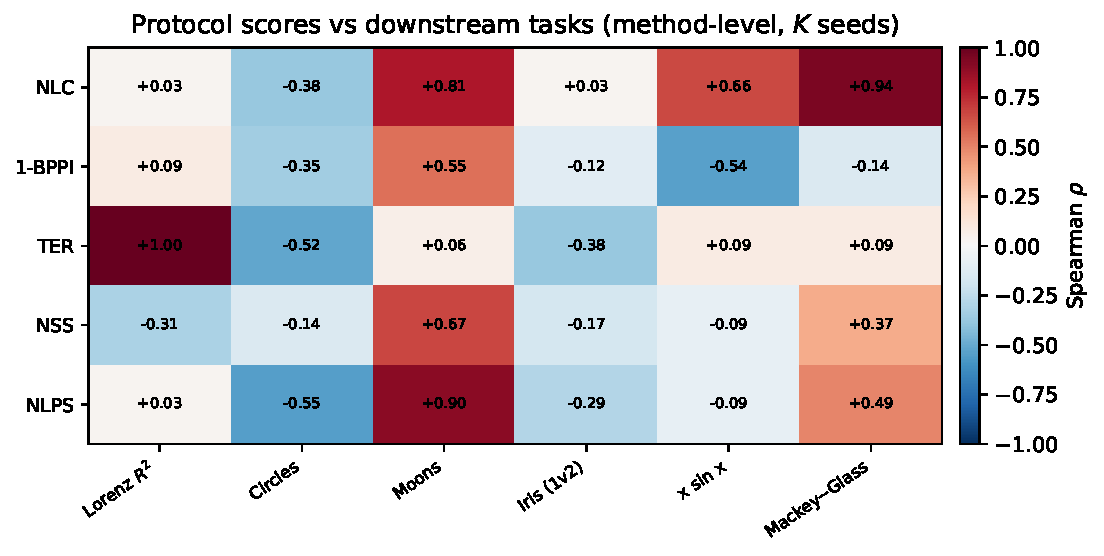
\includegraphics[width=\linewidth]{protocol_downstream_corr.pdf}
  \caption{Heatmap of Spearman $\rho$ between protocol scalars and downstream task scores (method-level means, $K=5$ seeds).}
  \label{fig:downstream-corr}
\end{figure}

\section{Ansatz taxonomy and protocol extensions}
\label{app:ansatz-taxonomy}

Table~\ref{tab:ansatz-taxonomy} maps common non-linearity mechanism classes to the reference registry rows and states whether the current release evaluates them under the fixed \nlc/\bppi/\nss/\ter\ stages.
The six quantum rows were chosen to \emph{isolate} one mechanism each (encoding, channel, both, hardware-efficient entanglement, hierarchy, fixed random dynamics) while keeping parameter counts comparable; classical and hybrid rows are non-competing references.
Mid-circuit measurements with feed-forward, quantum kernels without trainable \pqcs, and native open-system training are out of scope for the reference tables but can be added by registering a builder and rerunning the same stage order once simulator support and resource accounting are in place.

\begin{table}[t]
  \caption{Non-linearity mechanism classes and their status in the reference protocol.}
  \label{tab:ansatz-taxonomy}
  \centering
  \footnotesize
  \begin{tabular}{p{0.34\linewidth}p{0.28\linewidth}p{0.30\linewidth}}
    \toprule
    Mechanism class & Reference row & Status \\
    \midrule
    Data reuploading / encoding & Data reuploading & Included \\
    CPTP channel (ancilla trace) & Ancilla tracing, ancilla reuploading & Included \\
    Hardware-efficient entanglement & Strongly entangling (baseline) & Included \\
    Hierarchical structure & Quantum CNN & Included \\
    Fixed random features + readout & Quantum reservoir & Included \\
    Classical activations & Classical MLP (ref.) & Reference only \\
    Hybrid circuit + classical layer & Hybrid QCNN (ref.) & Reference only \\
  \midrule
    Mid-circuit measurement + feed-forward & --- & Excluded (branching simulator, readout noise accounting) \\
    Nonlinear classical readout only & Hybrid (partial) & Partial via hybrid reference \\
    Quantum kernels (no trainable \pqc) & --- & Out of scope (different hypothesis class) \\
    Native open-system training & --- & Future (NSS uses post-hoc depolarizing on trained unitary models) \\
    \bottomrule
  \end{tabular}
\end{table}

\section{BPPI probe-loss ablation}
\label{app:bppi-probe-ablation}

\bppi\ is computed from a scalar probe loss shared across methods (Appendix~\ref{app:reproducibility}), so cross-method rankings can reflect the probe as well as the ansatz.
We re-estimate $1-\bppi$ under alternate probes at $(n,L)=(3,3)$ with ablation budget $N_{\mathrm{init}}=16$, $n\in\{2,4,6\}$, and seeds $\{42,43\}$ (the published default stage uses $N_{\mathrm{init}}=256$, $n\in\{2,4,6,8\}$).
As a control, we also re-run the default probe at that same ablation budget.
Table~\ref{tab:bppi-probe-ablation} reports Kendall $\tau$ of each ranking against the published default on the same seeds.
The control itself has $\tau = 0.47$ against the published default, so mid-rank movement at this budget is within estimation noise; strongly entangling layers remain last under the cheap default and under every alternate probe.
The claim the ablation supports is therefore the plateau-risk verdict, not a fine ordering within the low-risk group.

% Auto-generated by scripts/bppi_probe_ablation.py
\begin{table}[t]
  \caption{BPPI rank bands under alternate probe losses at $(n,L)=(3,3)$. Ablation budget: $N_{\mathrm{init}}=16$, $n\in\{2,4,6\}$, seeds 42, 43. Ranks follow $1-\mathrm{BPPI}$ (higher is better). Kendall $\tau$ is against the published default probe (full stage: $N_{\mathrm{init}}=256$, $n\in\{2,4,6,8\}$) on the same seeds. The row \texttt{default (ablation budget)} re-runs the default probe at the ablation budget as a control.}
  \label{tab:bppi-probe-ablation}
  \centering
  \footnotesize
  \begin{tabular}{lrrl}
    \toprule
    Probe & Kendall $\tau$ vs published default & Top method & Bottom two (ranks 5--6) \\
    \midrule
    default (published) & 1.00 & ancilla tracing & quantum reservoir, strongly entangling \\
    default (ablation budget) & 0.47 & ancilla reuploading & qcnn, strongly entangling \\
    alt $x{=}0.1$ & 0.87 & ancilla reuploading & quantum reservoir, strongly entangling \\
    alt $x{=}1.0$ & 0.60 & data reuploading & quantum reservoir, strongly entangling \\
    local $\sin$ MSE & 0.60 & ancilla reuploading & quantum reservoir, strongly entangling \\
    \bottomrule
  \end{tabular}
\end{table}


\section{Scaling at $(n,L)=(4,4)$}
\label{app:scaling-n4-l4}

To test whether composite rankings depend on a single operating point, we repeat the full protocol at $(n,L)=(4,4)$ with the same seed set and training budgets as the $(3,3)$ reference run ($K=5$).
% Composite columns from scripts/paper_export_scaling_table.py (results/scaling_comparison/summary.json).
% Component columns transcribed from the authors' OpenReview rebuttal of 27 Jul 2026 (same (4,4) run, K=5, seeds 42-46);
% the per-seed sweep directories are not kept in the repository, so the script cannot regenerate them.
% Kendall tau between (n,L)=(3,3) and (4,4) mean NLPS ranks: 0.600
\begin{table}[t]
  \caption{Mean component and composite scores at $(n,L)=(3,3) \rightarrow (4,4)$ (quantum ans\"atze only, $K=5$ seeds), with the \nlps\ rank at each point. Kendall $\tau=0.60$ between the two rank orderings.}
  \label{tab:scaling-n4-l4}
  \centering
  \footnotesize
  \setlength{\tabcolsep}{4pt}
  \resizebox{\textwidth}{!}{%
  \begin{tabular}{lcccccc}
    \toprule
    Method & \nlc & $1-\bppi$ & \ter & \nss & \nlps & Rank $(3,3)\rightarrow(4,4)$ \\
    \midrule
    Data reuploading    & $0.437 \rightarrow 0.582$ & $0.876 \rightarrow 0.666$ & $0.073 \rightarrow 0.118$ & $0.902 \rightarrow 0.825$ & $0.567 \rightarrow 0.559$ & $1 \rightarrow 2$ \\
    Ancilla tracing     & $0.307 \rightarrow 0.125$ & $0.988 \rightarrow 0.813$ & $0.088 \rightarrow 0.088$ & $0.893 \rightarrow 0.844$ & $0.551 \rightarrow 0.433$ & $2 \rightarrow 4$ \\
    Ancilla reuploading & $0.261 \rightarrow 0.593$ & $0.938 \rightarrow 0.861$ & $0.151 \rightarrow 0.122$ & $0.673 \rightarrow 0.761$ & $0.491 \rightarrow 0.599$ & $3 \rightarrow 1$ \\
    Quantum CNN         & $0.292 \rightarrow 0.374$ & $0.662 \rightarrow 0.448$ & $0.121 \rightarrow 0.125$ & $0.890 \rightarrow 0.856$ & $0.470 \rightarrow 0.439$ & $4 \rightarrow 3$ \\
    Strongly entangling & $0.368 \rightarrow 0.427$ & $0.029 \rightarrow 0.035$ & $0.123 \rightarrow 0.111$ & $0.338 \rightarrow 0.482$ & $0.228 \rightarrow 0.277$ & $5 \rightarrow 5$ \\
    Quantum reservoir   & $0.087 \rightarrow 0.100$ & $0.311 \rightarrow 0.310$ & $0.009 \rightarrow 0.008$ & $0.517 \rightarrow 0.516$ & $0.213 \rightarrow 0.217$ & $6 \rightarrow 6$ \\
    \bottomrule
  \end{tabular}}
\end{table}

The bottom two ranks (strongly entangling layers and quantum reservoir) are unchanged; no method crosses between the top four and the bottom two.
Kendall $\tau$ between the two \nlps\ orderings is $0.60$, and the composite leader flips from data reuploading to ancilla reuploading.
Ancilla reuploading's climb is driven by \nlc\ ($0.261 \rightarrow 0.593$), not by \ter\ (which falls slightly, $0.151 \rightarrow 0.122$).
Ancilla tracing is the sole method whose \nlc\ collapses ($0.307 \rightarrow 0.125$): across all five seeds, $R^2(k{=}1)$ stays near one at both operating points, while $R^2(k{=}2)$ falls from about $0.73$ at $(3,3)$ to about $0$ at $(4,4)$, so under the fixed \nlc\ budget the pure channel mechanism reaches only the fundamental at $(4,4)$.
Because \bppi\ is measured on the fixed qubit sweep $n\in\{2,4,6,8\}$ regardless of the operating point, the $1-\bppi$ column of this comparison varies with depth $L$ alone.
These results motivate reading \nlps\ as a rank-band summary within a declared $(n,L)$, not across operating points.

\section{Weight sensitivity Monte Carlo}
\label{app:weight-sensitivity}

The composite \nlps\ in~\eqref{eq:nlps-formula} and the internal \ter\ combination in~\eqref{eq:ter-formula} are weighted based on fixed conventions, so we ask how large the impact of the weights is on the \emph{ordering} of methods rather than on the underlying component scores in Table~\ref{tab:nlps-components}.
We analyze this by holding the component scores fixed at their reference-run values and performing Monte Carlo resampling of the weights only without retraining any of the circuits.

\paragraph{Resampled \nlps\ weights.}
We draw $10^5$ independent weight vectors $(w_{\nlc}, w_{1-\bppi}, w_{\ter}, w_{\nss})$ from two families.
\emph{Global admissible weights} are sampled by drawing $u\sim\mathrm{Dirichlet}(1,1,1,1)$, setting $w_i=0.15+0.40u_i$, and retaining only draws satisfying $w_{\nlc} > w_{1-\bppi} \geq w_{\ter}$ and $w_{\nlc} > w_{1-\bppi} \geq w_{\nss}$, encoding the same priority ordering as the prose rationale for~\eqref{eq:nlps-formula}.
\emph{Local perturbations} take $\|w - w^{(0)}\|_\infty \leq \varepsilon$ around the published vector $w^{(0)} = (0.35, 0.25, 0.20, 0.20)$ with the same inequalities and simplex constraint; operationally, we sample perturbations in the first three coordinates, set the fourth coordinate so the weights sum to one, and reject samples outside the $\ell_\infty$ ball or the priority cone.
We use $\varepsilon \in \{0.05, 0.10, 0.15\}$ and report the $\varepsilon = 0.10$ case in the text.
Randomness uses a fixed seed so the experiment is reproducible.
For each sample we rank methods by the induced \nlps\ and record the empirical min-max rank per method over all $10^5$ samples.

\paragraph{Resampled \ter\ weights.}
We likewise draw $10^5$ triples $(w_{A}, w_{b}, w_{t})$ for the train-curve area, best train skill, and final test skill in~\eqref{eq:ter-formula}, rejecting unless $w_{A} > w_{b} > w_{t}$, $w_{A} \geq 0.40$, $w_{t} \geq 0.10$, and $\sum_i w_i = 1$.
Each triple is applied to the stored \ter\ sub-scores and the published parameter-efficiency multiplier, so \ter\ is recomputed without re-running Lorenz training.
We then substitute the perturbed \ter\ into~\eqref{eq:nlps-formula} while keeping the other three \nlps\ components and the published $(0.35, 0.25, 0.20, 0.20)$ fixed, to see whether \ter-only uncertainty can reorder the composite.

\paragraph{Outcomes.}
Table~\ref{tab:weight-sensitivity-nlps} summarizes the \nlps\ rank bands under global admissible weights; the local-$\varepsilon$ runs give the same bands for ranks $1$-$2$ and differ only slightly in the middle pair (ancilla reuploading versus \textsc{qcnn} still occupy ranks $3$-$4$ only).
The mean Kendall $\tau$ correlation between the per-sample full ranking and the published ranking is $0.974$ under global sampling and $0.982$ at $\varepsilon = 0.10$.
To quantify how far one must move from the published coefficients before a rank change is possible, we also solve the local tie constraints exactly under the same priority inequalities.
The nearest rank tie is between ancilla reuploading and \textsc{qcnn} at $\|w-w^{(0)}\|_\infty \approx 0.015$; the bottom pair (strongly entangling layers versus quantum reservoir) can tie at distance $\approx 0.042$; by contrast, the top pair (data reuploading versus ancilla tracing) cannot be reversed within the stated priority cone, and ancilla tracing versus ancilla reuploading requires a much larger local move of about $0.181$.
Under \ter-only resampling, ancilla reuploading remains top-\ter\ in every draw, while \textsc{qcnn} and strongly entangling layers swap ranks $2$ and $3$ in about $41\%$ and $59\%$ of draws respectively; nevertheless, propagating those \ter\ draws into~\eqref{eq:nlps-formula} leaves the full six-way \nlps\ order identical to Table~\ref{tab:nlps-components} on every sample for the reference components.
These checks support reading the headline composite as stable under the stated weight priors, while treating the ancilla reuploading versus \textsc{qcnn} gap as a rank band rather than a knife-edge ordering.

\begin{table}[t]
  \caption{Empirical min-max \nlps\ rank of each method over $10^5$ Monte Carlo draws of globally admissible \nlps\ weights (Appendix~\ref{app:weight-sensitivity}). Ranks follow Table~\ref{tab:nlps-components} (higher \nlps\ is better).}
  \label{tab:weight-sensitivity-nlps}
  \centering
  \small
  \begin{tabular}{lcc}
    \toprule
    Method & min rank & max rank \\
    \midrule
    Data reuploading & 1 & 1 \\
    Ancilla tracing & 2 & 2 \\
    Ancilla reuploading & 3 & 4 \\
    Quantum CNN & 3 & 4 \\
    Strongly entangling & 5 & 6 \\
    Quantum reservoir & 5 & 6 \\
    \bottomrule
  \end{tabular}
\end{table}

\newpage
\section*{NeurIPS Paper Checklist}

\begin{enumerate}

\item {\bf Claims}
    \item[] Question: Do the main claims made in the abstract and introduction accurately reflect the paper's contributions and scope?
    \item[] Answer: \answerYes{}
    \item[] Justification: The abstract and the contributions list in Section~\ref{sec:introduction} state three scoped claims---a four-axis protocol with a composite index (developed in Section~\ref{sec:protocol}), a reference evaluation of six quantum ans\"atze (Sections~\ref{sec:protocol-results}--\ref{sec:real-data-results}), and an empirical diagnosis of metric divergence (Section~\ref{sec:metric-divergence})---each of which is demonstrated in the indicated section and not stronger than what the experiments support. The paper does not claim a new quantum algorithm, a new model, or hardware results.

\item {\bf Limitations}
    \item[] Question: Does the paper discuss the limitations of the work performed by the authors?
    \item[] Answer: \answerYes{}
    \item[] Justification: Section~\ref{sec:limitations} lists the main ones: fixed optimization budget on hard chaotic regressions, depolarizing noise as a proxy for real hardware error channels, a reference operating point of $(n,L) = (3,3)$ with a single $(4,4)$ repeat (Appendix~\ref{app:scaling-n4-l4}) showing that composite rank bands do not transfer across operating points, the probe-loss dependence of \bppi\ (Appendix~\ref{app:bppi-probe-ablation}), and the scope restriction to unitary ans\"atze with expectation-value readouts. Section~\ref{sec:problem-formulation} separately discusses the reasons mid-circuit measurement and feed-forward mechanisms are outside the reference registry.

\item {\bf Theory assumptions and proofs}
    \item[] Question: For each theoretical result, does the paper provide the full set of assumptions and a complete (and correct) proof?
    \item[] Answer: \answerNA{}
    \item[] Justification: The paper does not state theorems or proofs. The equations in Section~\ref{sec:protocol} are metric \emph{definitions} whose design rationale and coefficient choices are discussed in-place and in Appendix~\ref{app:metric-details}.

\item {\bf Experimental result reproducibility}
    \item[] Question: Does the paper fully disclose all the information needed to reproduce the main experimental results of the paper to the extent that it affects the main claims and/or conclusions of the paper?
    \item[] Answer: \answerYes{}
    \item[] Justification: Section~\ref{sec:methods} fixes all training details (task sizes, optimizer, learning rate, optimization budgets, qubit and layer counts, the barren-plateau qubit sweep, and the noise ladder). Appendix~\ref{app:metric-details} gives the per-metric artifact manifest and the run-fingerprint convention used to invalidate cached partial runs. The source code, metric definitions, seeds, and per-seed raw diagnostics are publicly released at the repository named in Appendix~\ref{app:reproducibility}.

\item {\bf Open access to data and code}
    \item[] Question: Does the paper provide open access to the data and code, with sufficient instructions to faithfully reproduce the main experimental results, as described in supplemental material?
    \item[] Answer: \answerYes{}
    \item[] Justification: The full evaluation pipeline (circuit registry, metric implementations, plotting and table-export scripts, and pre-computed per-seed raw diagnostics) is publicly released at the repository named in Appendix~\ref{app:reproducibility} (the same code was provided as the supplement during review). A top-level driver runs the protocol end-to-end; the required commands, environment specification, and expected outputs are included in the repository README. All datasets used (Lorenz, Mackey--Glass, scikit-learn \textsc{circles}/\textsc{moons}/Iris) are either synthesized by the released code or loaded from publicly available sources.

\item {\bf Experimental setting/details}
    \item[] Question: Does the paper specify all the training and test details necessary to understand the results?
    \item[] Answer: \answerYes{}
    \item[] Justification: Section~\ref{sec:methods} fixes the optimizer (Adam), the learning rate, the training-set and evaluation-set sizes, the step budgets (including the per-method step boosts documented with the release), the random seed convention, the qubit-sweep and noise-ladder parameters, and the split used for the hybrid baseline.

\item {\bf Experiment statistical significance}
    \item[] Question: Does the paper report error bars suitably and correctly defined or other appropriate information about the statistical significance of the experiments?
    \item[] Answer: \answerYes{}
    \item[] Justification: Tables~\ref{tab:nlps-components}--\ref{tab:real-data} report mean $\pm$ one standard deviation across random-seed replicates of the full protocol (the number of seeds $K$ is stated in the aggregation blurb appended to each caption). The factor of variability is the global random seed (\texttt{QNLEP\_SEED}), which controls parameter initialization, the Lorenz train/test split, the barren-plateau initialization ensemble, and the quantum-reservoir random unitary. Standard deviations are computed across seeds using the standard unbiased estimator; with a single seed the tables fall back to point estimates, which is stated in the caption.

\item {\bf Experiments compute resources}
    \item[] Question: For each experiment, does the paper provide sufficient information on the computer resources needed to reproduce the experiments?
    \item[] Answer: \answerYes{}
    \item[] Justification: The ``Compute footprint'' subsection in Appendix~\ref{app:reproducibility} reports that the full protocol at $(n, L) = (3, 3)$ runs in approximately two hours of wall time on a single eight-core consumer CPU (no GPU) and that a five-seed sweep completes overnight on the same machine; the $(4,4)$ repeat (Appendix~\ref{app:scaling-n4-l4}) has the same per-seed cost, and the probe ablation (Appendix~\ref{app:bppi-probe-ablation}) runs at a reduced budget stated there. The barren-plateau sweep at $n = 8$ with $N_{\mathrm{init}} = 256$ is the dominant cost.

\item {\bf Code of ethics}
    \item[] Question: Does the research conducted in the paper conform, in every respect, with the NeurIPS Code of Ethics?
    \item[] Answer: \answerYes{}
    \item[] Justification: The work is a methodological contribution evaluated on textbook synthetic tasks (Lorenz, Mackey--Glass, sinusoidal ladders, and small classical benchmarks shipped with scikit-learn). It does not involve human subjects, personal data, crowdsourcing, pre-trained generative models, or scraped web content. Anonymity requirements were respected during review.

\item {\bf Broader impacts}
    \item[] Question: Does the paper discuss both potential positive societal impacts and negative societal impacts of the work performed?
    \item[] Answer: \answerYes{}
    \item[] Justification: Section~\ref{sec:conclusion} states that the protocol is an evaluation tool for a pre-deployment research community and that no dual-use concerns specific to it are identified.

\item {\bf Safeguards}
    \item[] Question: Does the paper describe safeguards that have been put in place for responsible release of data or models that have a high risk for misuse?
    \item[] Answer: \answerNA{}
    \item[] Justification: The only asset released is an evaluation pipeline together with its metric definitions, synthetic data loaders, and scalar scores; no generative model, pre-trained weights, or scraped dataset is released, and the assets carry no identifiable misuse profile beyond that of any open-source scientific code.

\item {\bf Licenses for existing assets}
    \item[] Question: Are the creators or original owners of assets used in the paper properly credited and are the license and terms of use explicitly mentioned and properly respected?
    \item[] Answer: \answerYes{}
    \item[] Justification: The ``Existing assets and licenses'' subsection in Appendix~\ref{app:reproducibility} credits PennyLane~\citep{bergholm2018pennylane} (Apache~2.0) for circuit simulation and scikit-learn~\citep{pedregosa2011scikitlearn} (BSD-3-Clause) for classical baselines and toy datasets; Lorenz~\citep{lorenz1963} and Mackey--Glass~\citep{mackeyglass1977} trajectories are generated from their canonical equations.

\item {\bf New assets}
    \item[] Question: Are new assets introduced in the paper well documented and is the documentation provided alongside the assets?
    \item[] Answer: \answerYes{}
    \item[] Justification: The new asset is the evaluation protocol itself, released as a pipeline with a method registry, metric implementations, synthetic data loaders, seed-indexed raw diagnostics, and an ordered driver script. The assets are documented in Appendix~\ref{app:metric-details} (per-metric reproducibility manifest, run-fingerprint convention) and in Section~\ref{sec:evaluation-protocol} (registration interface for new methods); intended use is scientific benchmarking of non-linearity mechanisms in variational quantum models.

\item {\bf Crowdsourcing and research with human subjects}
    \item[] Question: For crowdsourcing experiments and research with human subjects, does the paper include the full text of instructions given to participants and screenshots, if applicable, as well as details about compensation?
    \item[] Answer: \answerNA{}
    \item[] Justification: The paper does not involve crowdsourcing or research with human subjects.

\item {\bf Institutional review board (IRB) approvals or equivalent for research with human subjects}
    \item[] Question: Does the paper describe potential risks incurred by study participants, whether such risks were disclosed to the subjects, and whether Institutional Review Board (IRB) approvals (or an equivalent approval/review based on the requirements of your country or institution) were obtained?
    \item[] Answer: \answerNA{}
    \item[] Justification: The paper does not involve human subjects.

\item {\bf Declaration of LLM usage}
    \item[] Question: Does the paper describe the usage of LLMs if it is an important, original, or non-standard component of the core methods in this research?
    \item[] Answer: \answerNA{}
    \item[] Justification: LLMs are not a component of the method. The evaluated models are variational quantum circuits and a small classical multilayer perceptron baseline, none of which involve large language models. Any use of LLMs was limited to writing, editing, and formatting assistance, which per the checklist guidelines does not require a declaration.

\end{enumerate}


\end{document}
